\chapter{Manual d'usuari}


\section{Refer�ncies}

\begin{figure}[H]
\begin{center}
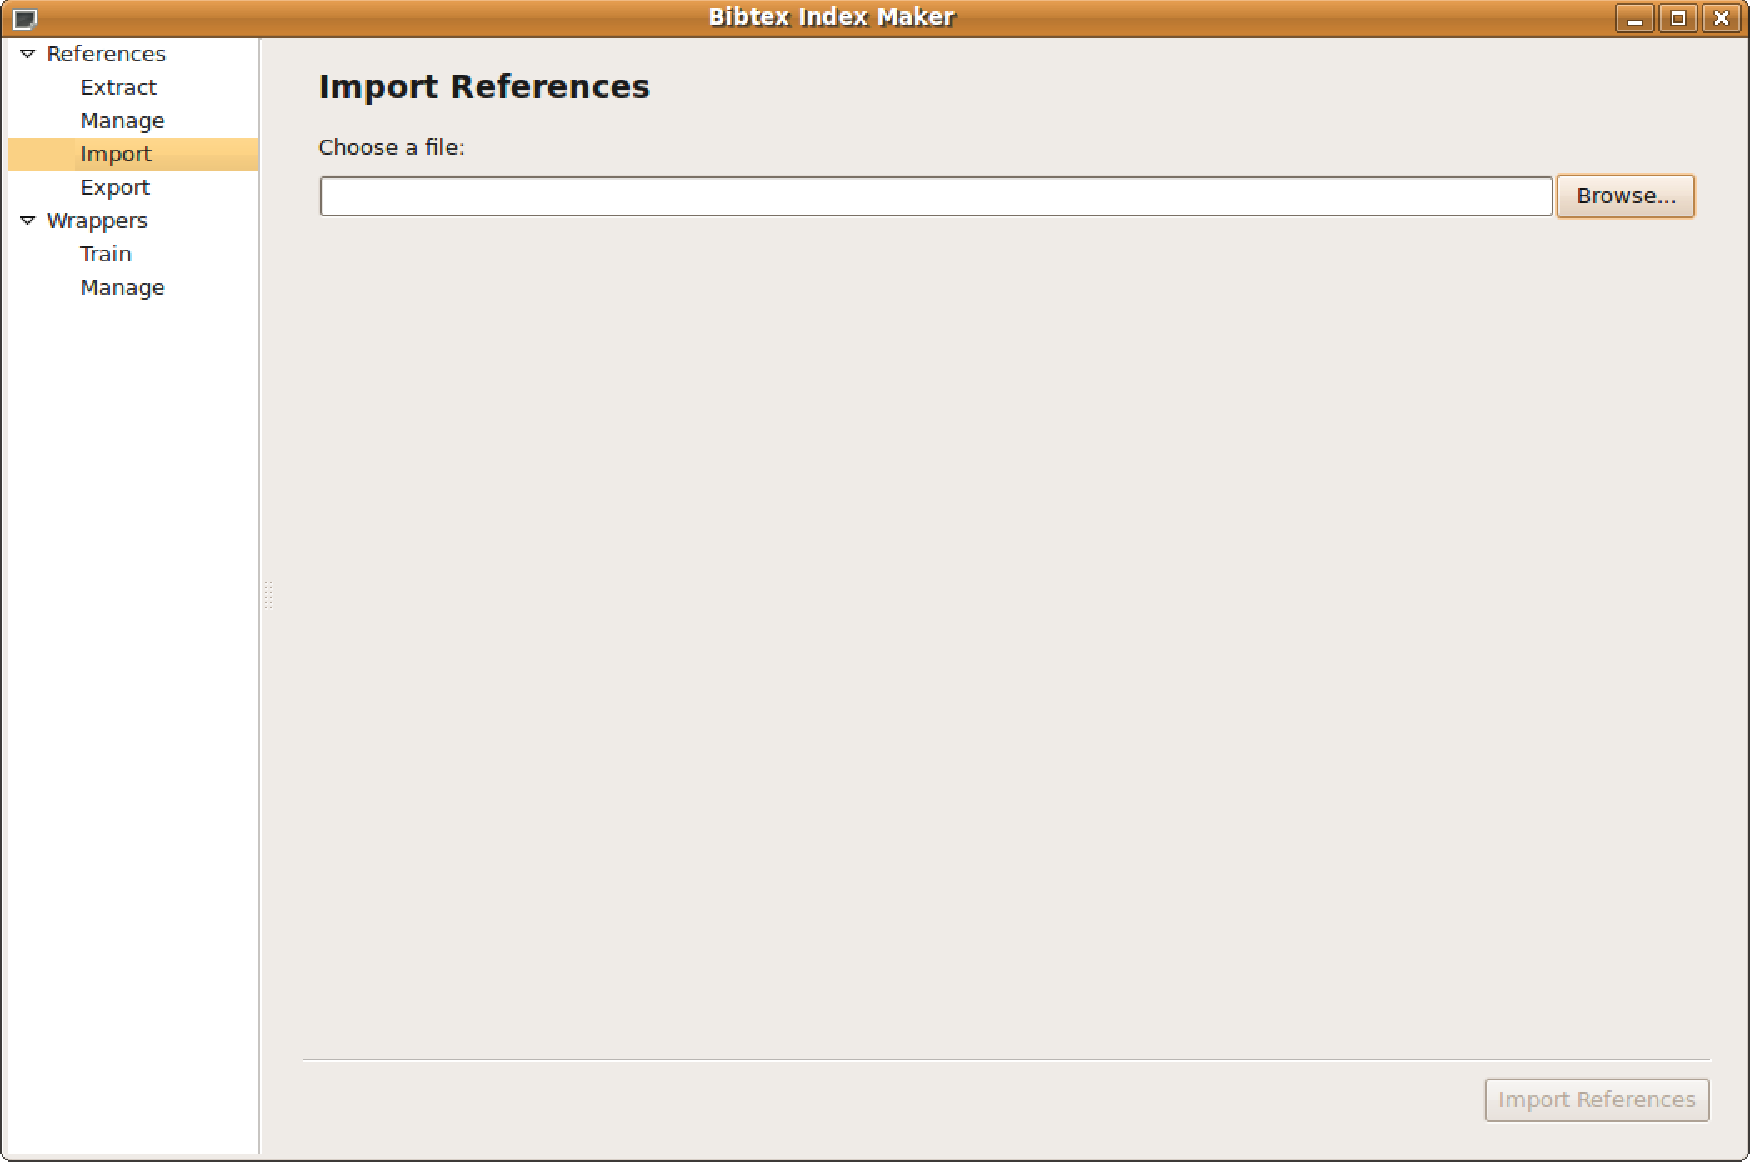
\includegraphics[width=0.9\textwidth]{figures/screenshots/screenshots:import-references.pdf}
\caption{Importa refer�ncies}
\label{fig:screenshots:import-references}
\end{center}
\end{figure}

Quan es clica comen�a el proc�s d'importaci� i es mostra la finestra. Per 

\begin{figure}[H]
\begin{center}
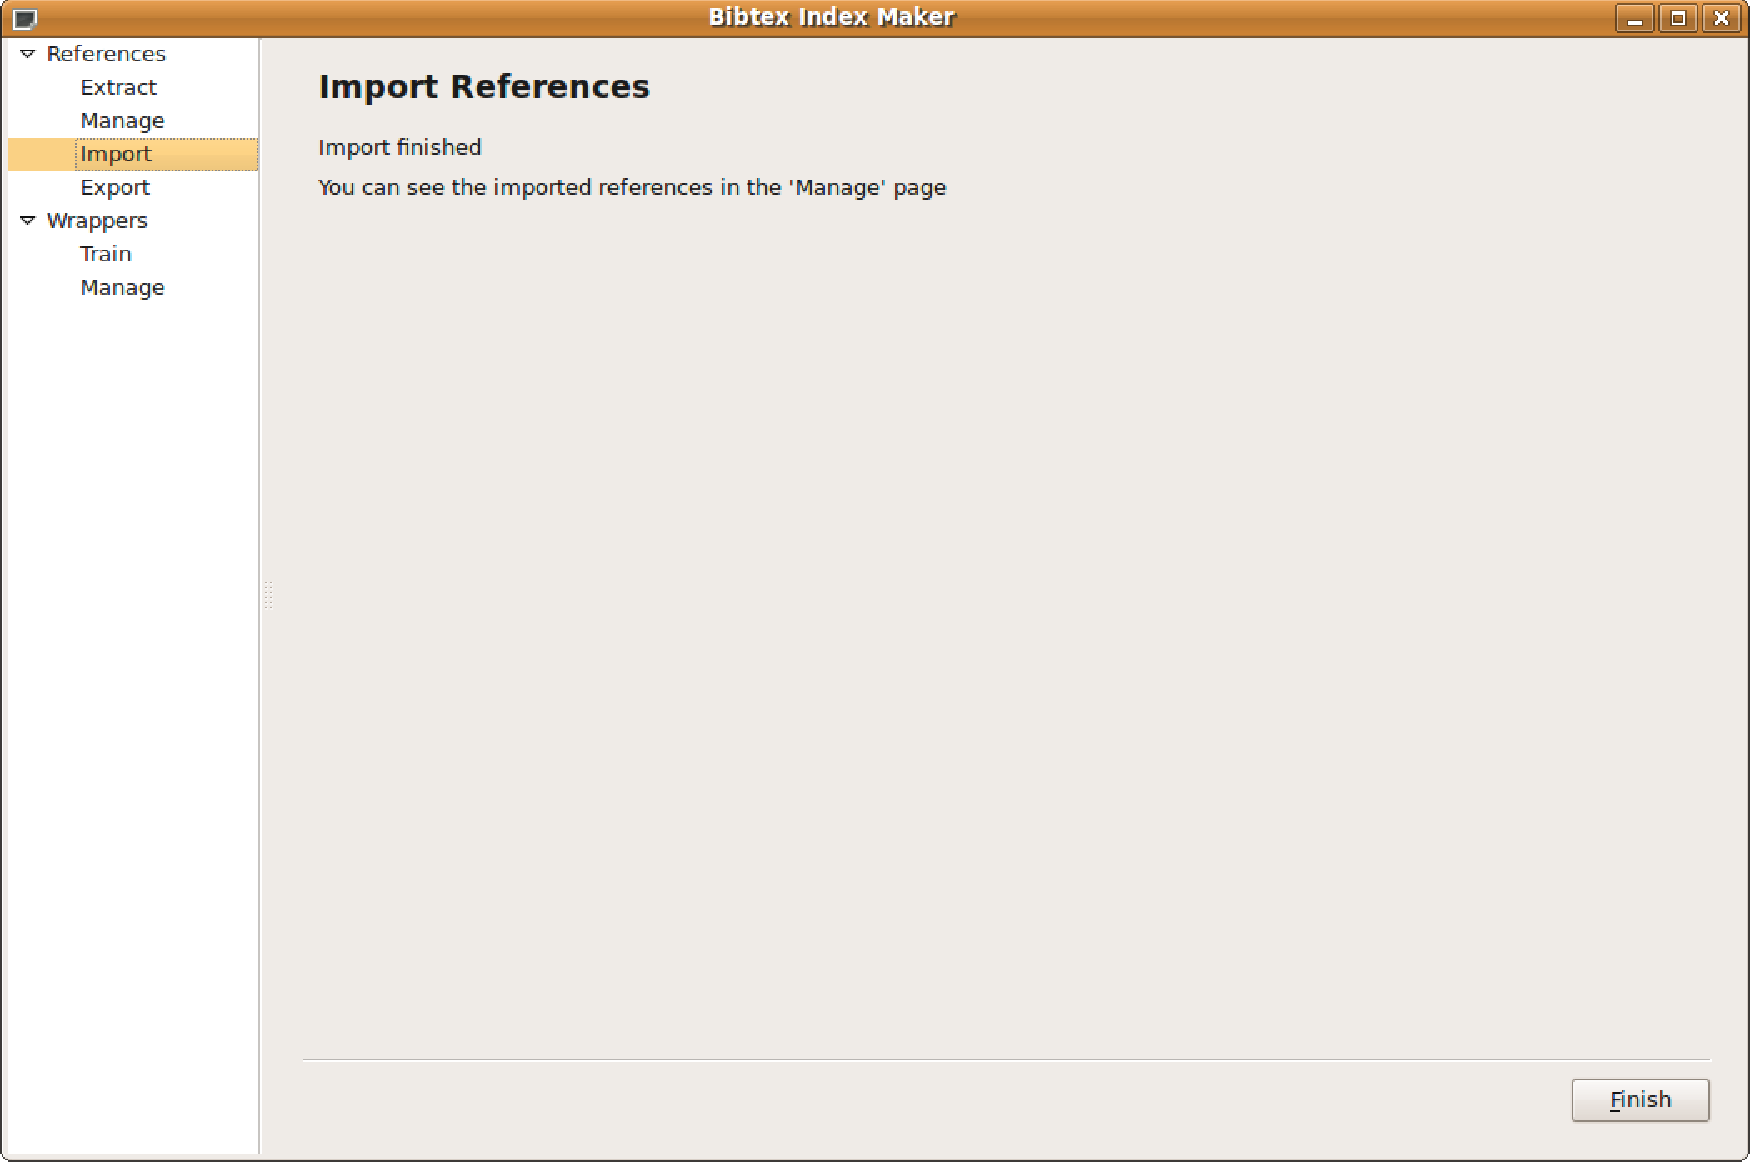
\includegraphics[width=0.9\textwidth]{figures/screenshots/screenshots:import-references-2.pdf}
\caption{Un cop s'han importat les refer�ncies}
\label{fig:screenshots:import-references-2}
\end{center}
\end{figure}


\begin{figure}[H]
\begin{center}
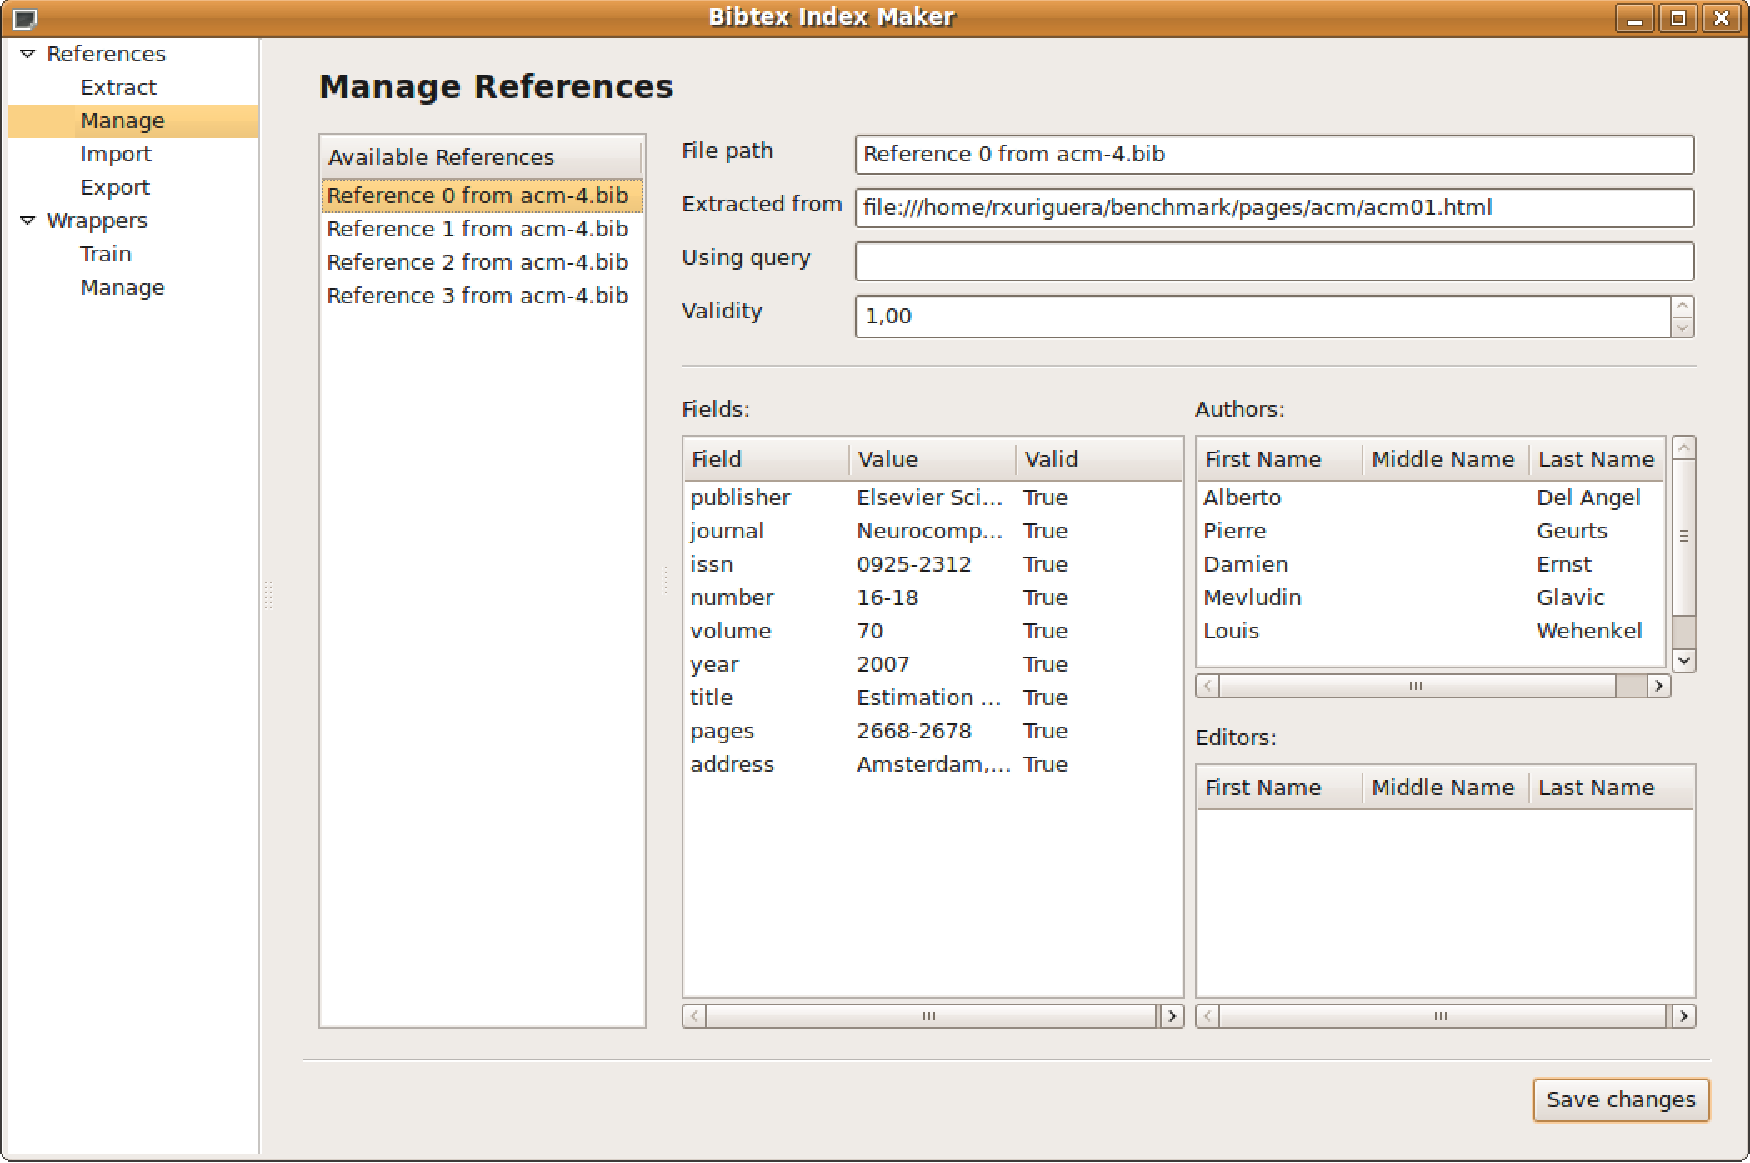
\includegraphics[width=0.9\textwidth]{figures/screenshots/screenshots:manage-references.pdf}
\caption{Maneig de refer�ncies}
\label{fig:screenshots:manage-references}
\end{center}
\end{figure}

\begin{figure}[H]
\begin{center}
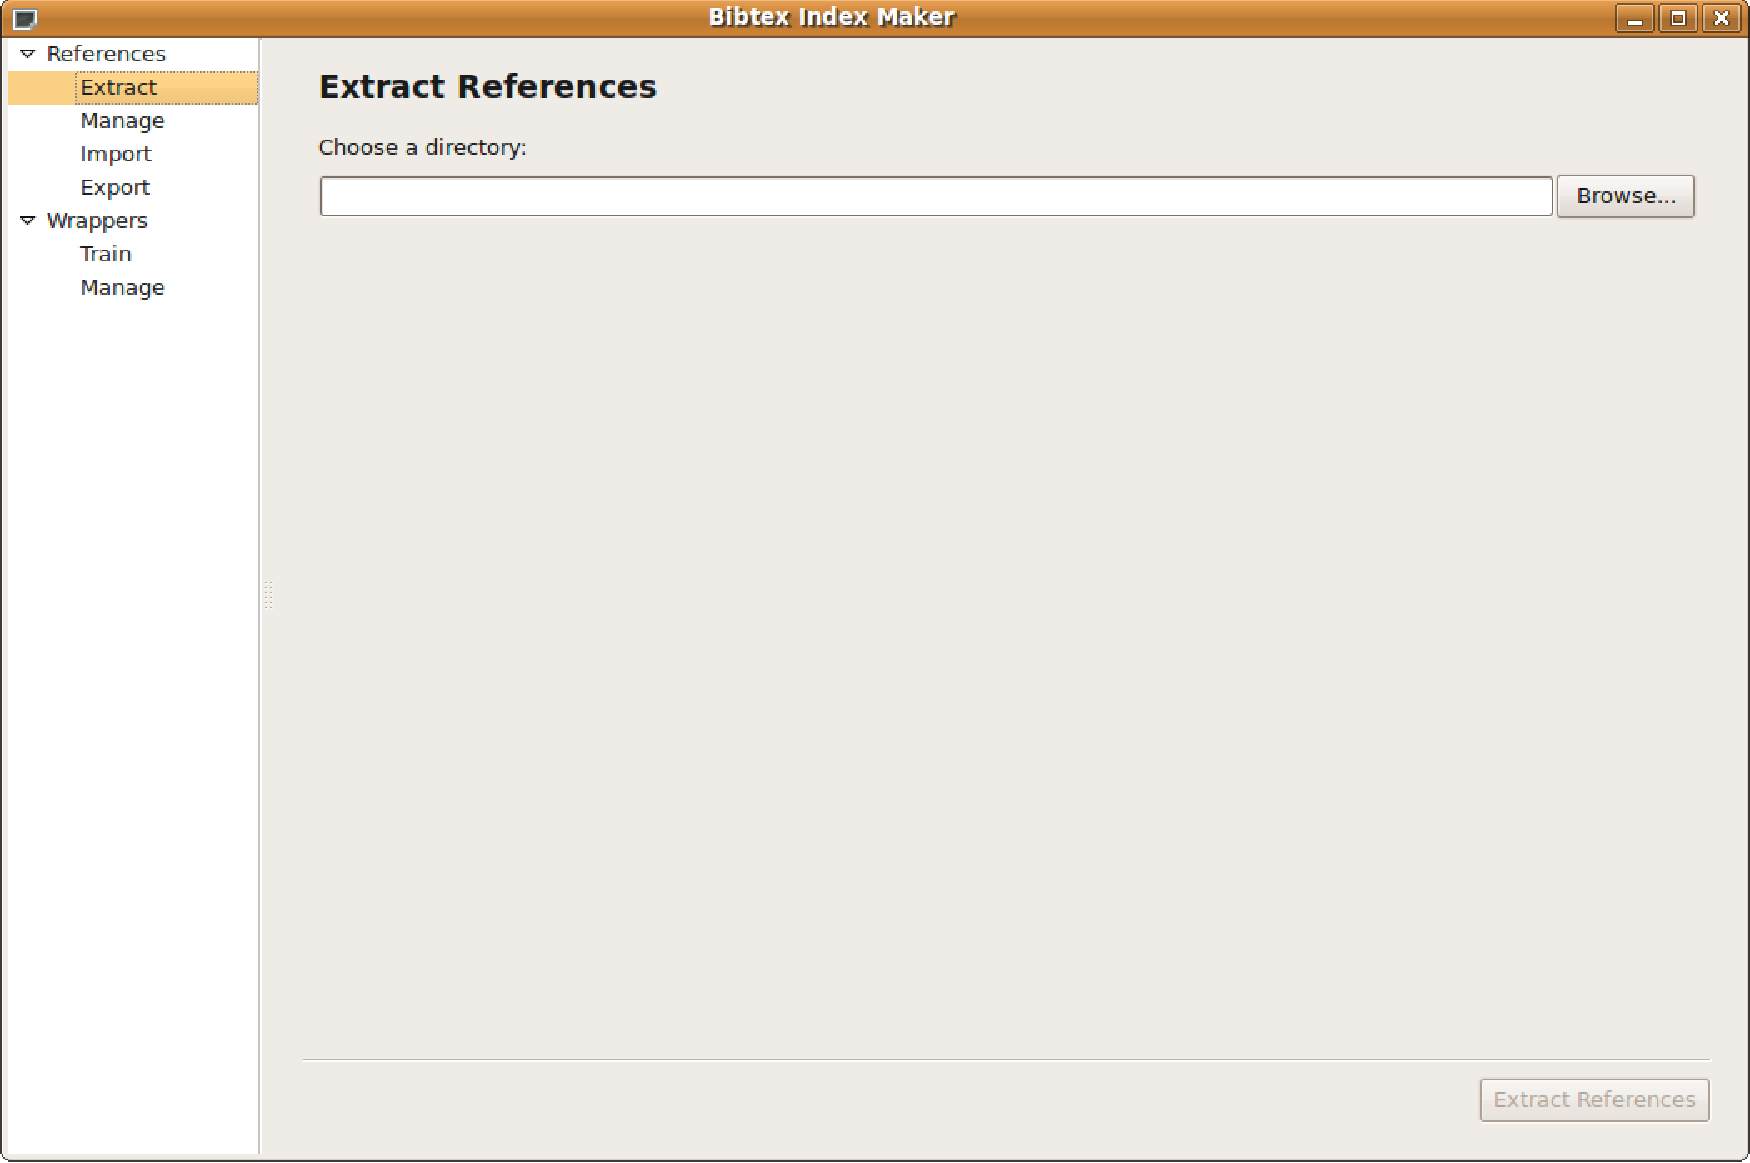
\includegraphics[width=0.9\textwidth]{figures/screenshots/screenshots:extract-references.pdf}
\caption{Extreu refer�ncies}
\label{fig:screenshots:extract-references}
\end{center}
\end{figure}



\begin{figure}[H]
\begin{center}
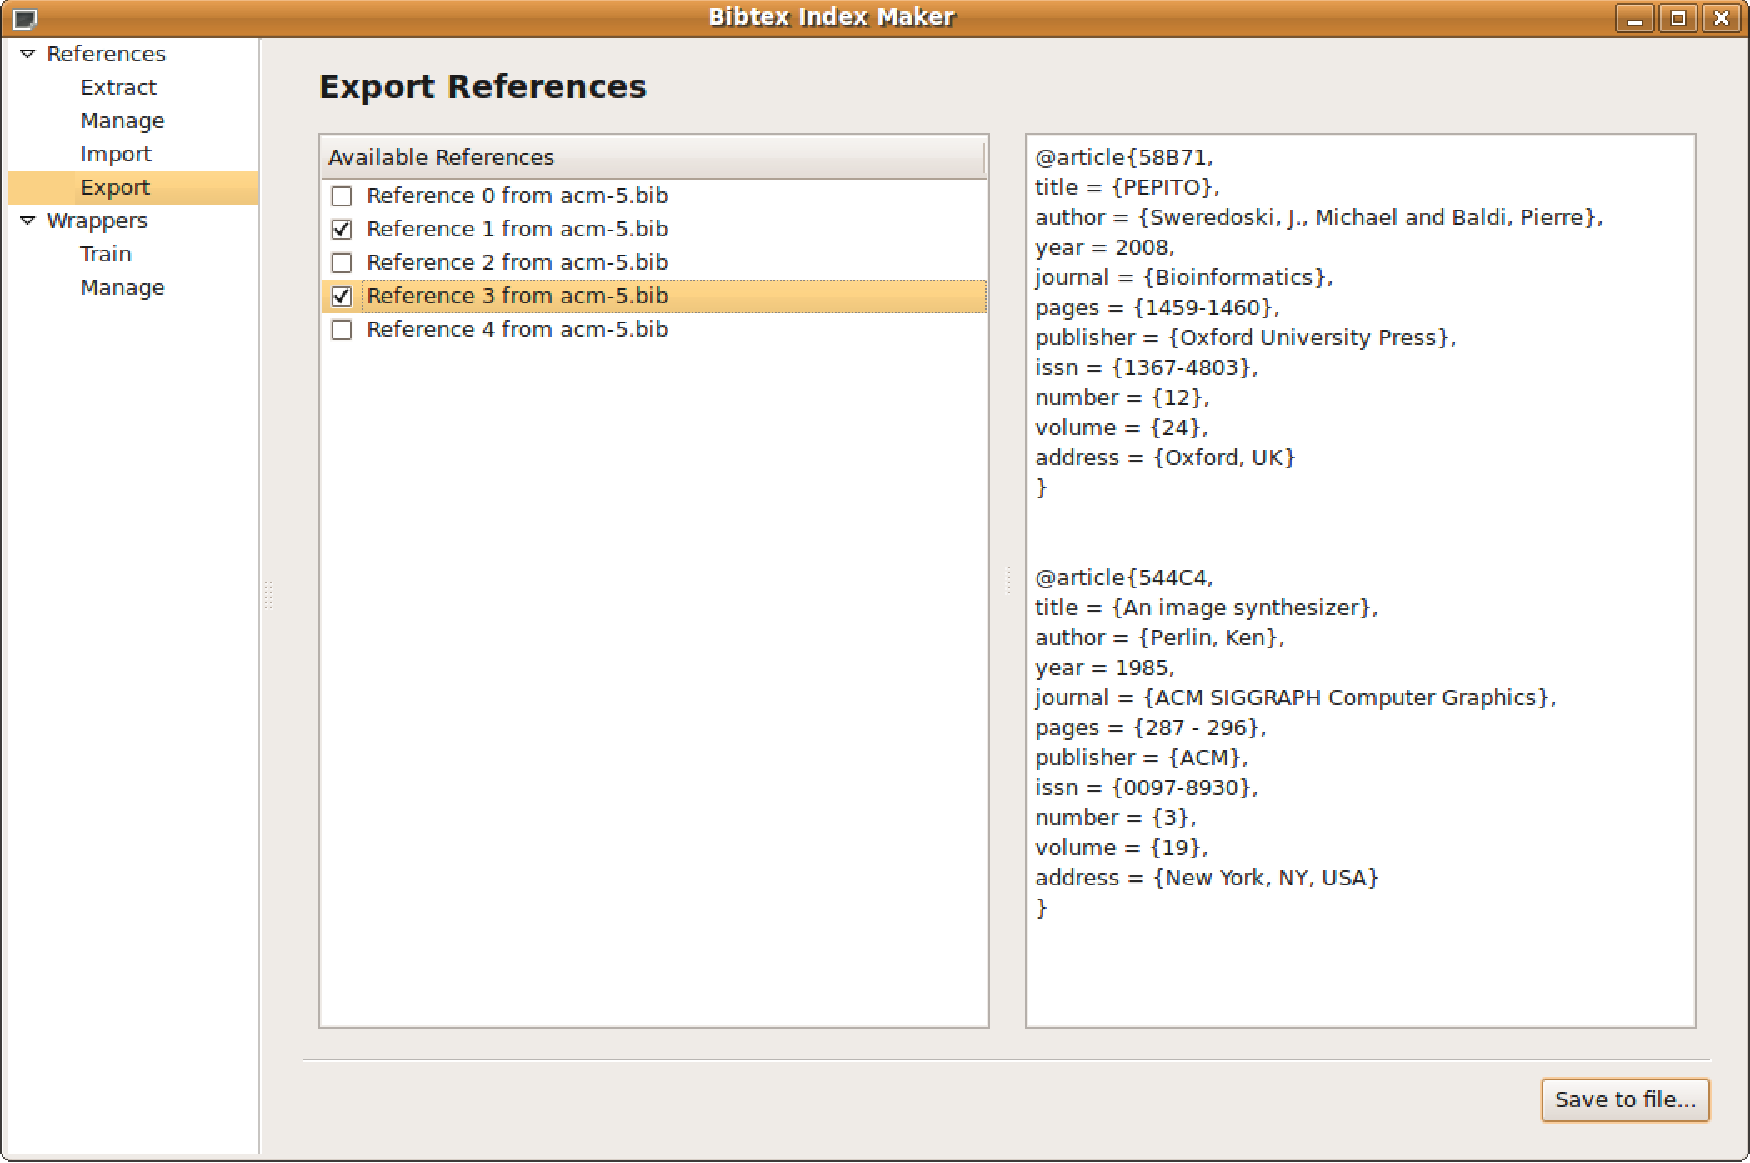
\includegraphics[width=0.9\textwidth]{figures/screenshots/screenshots:export-references.pdf}
\caption{Exporta refer�ncies}
\label{fig:screenshots:export-references}
\end{center}
\end{figure}


\section{\textit{Wrappers}}
Per poder extreure les refer�ncies, primer cal que tinguem \textit{wrappers} entrenats per les biblioteques digitals que m�s ens interessen. Per fer-ho, podem seleccionar l'opci� \textit{Train} del men� de l'aplicaci� i se'ns mostrar� la vista seg�ent.
\begin{figure}[H]
\begin{center}
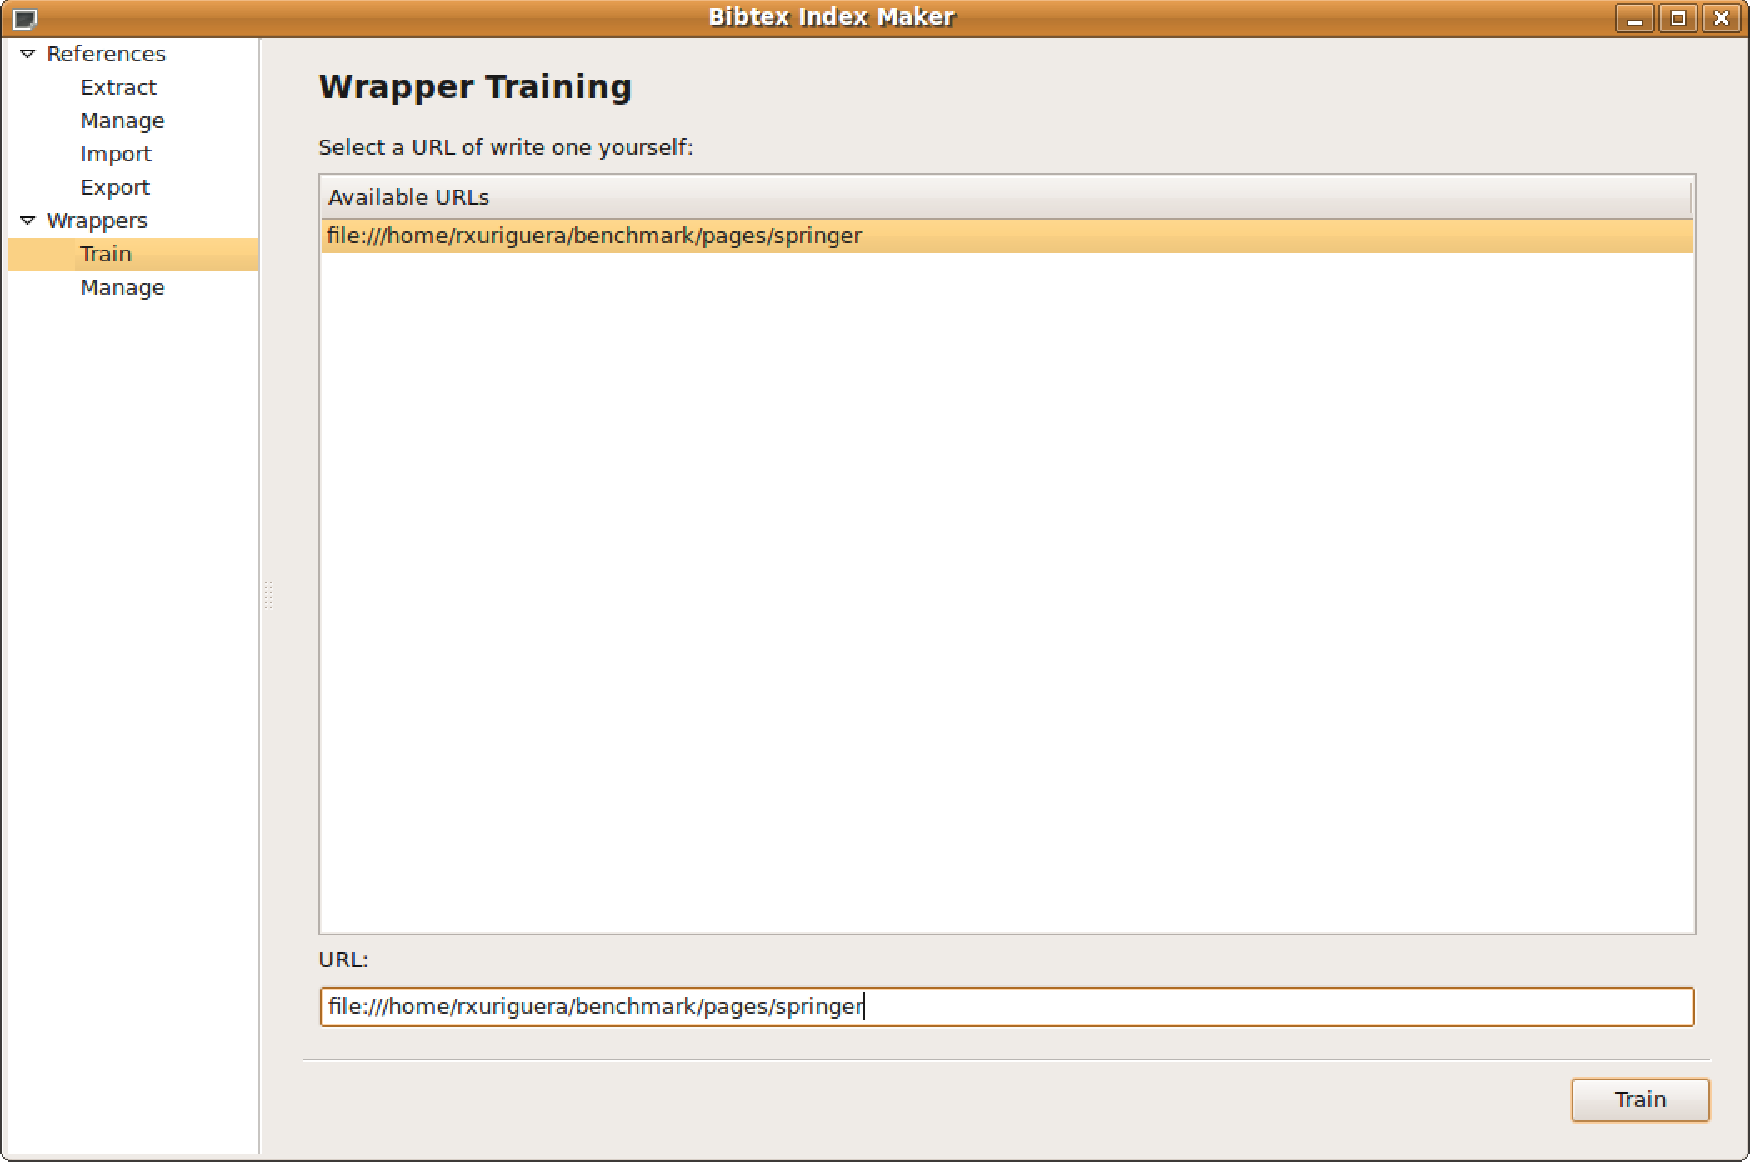
\includegraphics[width=0.9\textwidth]{figures/screenshots/screenshots:wrapper-train.pdf}
\caption{Entrenament de \textit{wrappers}}
\label{fig:screenshots:wrapper-train}
\end{center}
\end{figure}


Un cop hem generat els \textit{wrappers}, podem veure'ls i modificar-los a partir de l'opci� \textit{manage}, que ens porta a l'editor seg�ent. Des d'aqu� es poden realitzar les operacions CRUD per gestionar les col�leccions, \textit{wrappers} i les regles.
\begin{figure}[H]
\begin{center}
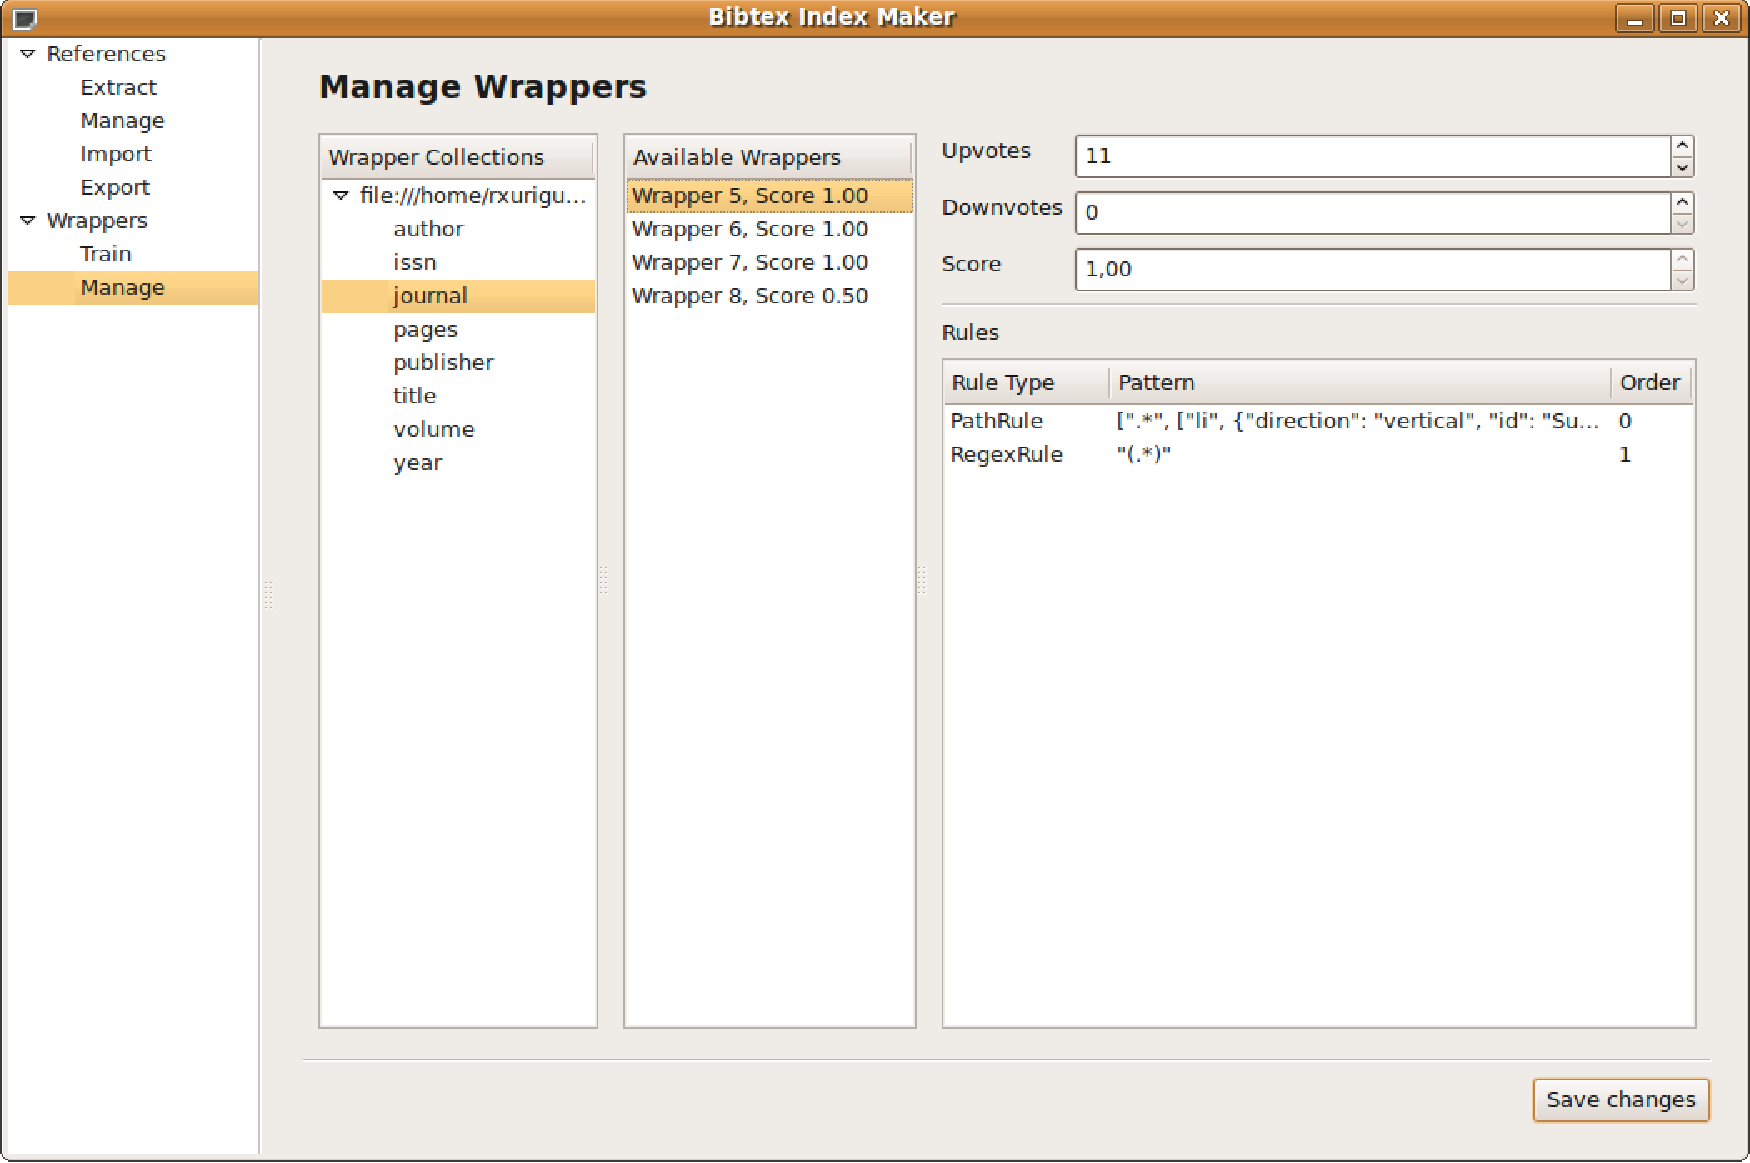
\includegraphics[width=0.9\textwidth]{figures/screenshots/screenshots:wrapper-manager.pdf}
\caption{Gesti� de \textit{wrappers}}
\label{fig:screenshots:wrapper-manager}
\end{center}
\end{figure}




